%Ordering Relation among Events----------------------------------------------------------------------------------------------------------------------       
\section{Ordering Relations among Events}
        
    %Agent Order
    \subsection{Agent Order ($\stck{_{ao}}$)}
        It is a union of total order among events belonging to the same agent event list. It is analogous to intra-thread ordering. For example, iftwo events $e$ and $d$ belong to the same agent event list , then either $\reln{e}{ao}{d}$ or $\reln{d}{ao}{e}$. 
        
        \begin{figure}[H]
            \centering
            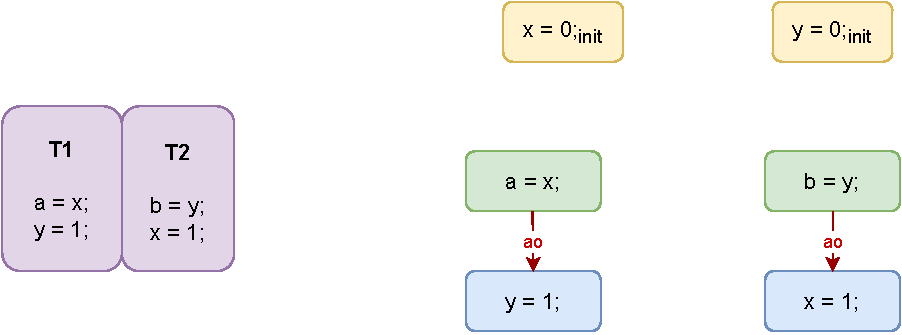
\includegraphics[scale=0.7]{4.ECMAScriptMemoryModel/AgentOrder.pdf}
            \caption{An example with agent order among the events.}
        \end{figure}
    
        %Synchronize With Order
    \subsection{Synchronize-With Order ($\stck{_{sw}} $)}
       Binary relation between two events that establish synchronization between multiple agents. It is a composition of two sets: 
        \begin{enumerate}
            \item All pairs belonging to $ASW$ of every agent belongs to this ordering relation. 
                \begin{align*}
                    \forall{i, j > 0}, \ \langle e_i, e_j \rangle \in ASW \Rightarrow{} \reln{e_i}{sw}{e_j} 
                \end{align*}
                    
            \item Specific reads-from pairs also belong to this ordering relation\footnotemark. 
                \begin{align*}
                    (\reln{r}{rf}{w}) \ \wedge \ \et{r}{sc} \ \wedge \ \et{w}{sc} \ \wedge \ (\Re(r)\!=\!\Re(w)) \ \Rightarrow{} \
                    (\reln{w}{sw}{r})
                \end{align*}
                    
        \end{enumerate}
        
        \begin{figure}[H]
            \centering
            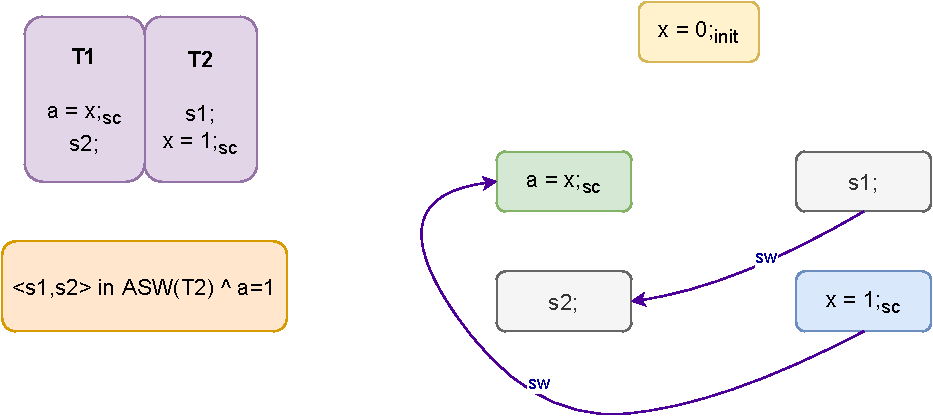
\includegraphics[scale=0.7]{4.ECMAScriptMemoryModel/SynchronizeWith.pdf}
            \caption{An example with synchronize with relations among the events.}
        \end{figure}

        \footnotetext{Note that for the second condition, both ranges of events have to be equal. This however, does not mean thatthe read cannot read from multiple write events. (the read-from relation here is not functional.)}
        
    %Happens Before order 
    \subsection{Happens Before Order ($\stck{_{hb}}$)}
        A transitive order on events, composed of the following:
        
        \begin{enumerate}
            \item Every agent-ordered relation is also a happens-before relation 
                \begin{align*}
                    (\reln{e}{ao}{d}) \ \Rightarrow{} \ (\reln{e}{hb}{d})    
                \end{align*}
                
            \item Every synchronize-with relation is also a happens-before relation 
                \begin{align*}
                    (\reln{e}{sw}{d}) \ \Rightarrow{} \ (\reln{e}{hb}{d})    
                \end{align*}
                 
            \item Initialize type of events happen before all shared memory events that have overlapping ranges with them. 
                \begin{align*}
                    \forall e,d \in SM \ \wedge \ 
                    \et{e}{init} \ \wedge \ 
                    (\Re(e) \cap \Re(d) \neq \phi)
                    \ \Rightarrow{} \ 
                    \reln{e}{hb}{d}
                \end{align*}          
        \end{enumerate}
    
        \begin{figure}[H]
            \centering
            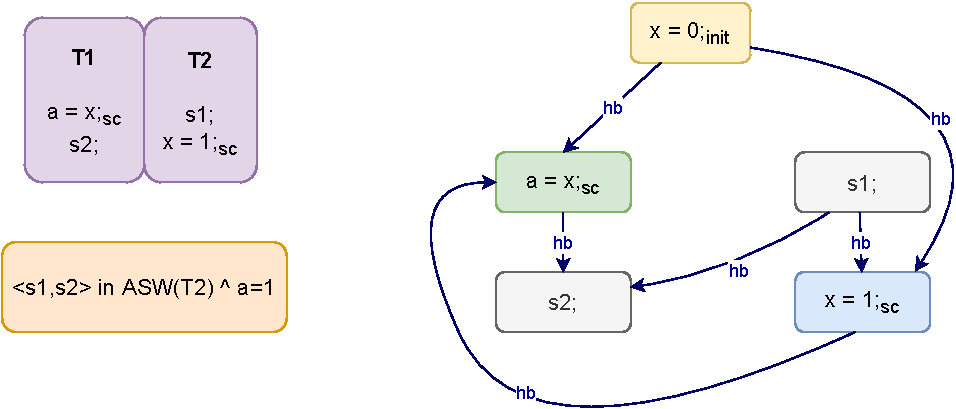
\includegraphics[scale=0.7]{4.ECMAScriptMemoryModel/Happens-before.pdf}
            \caption{An example with all the types of happens-before relations between events.}
        \end{figure}
    
    %Memory Order
    \subsection{Memory Order ($\stck{_{mo}}$)}
        A \textit{total order} on all events that respects happens-before order. 
        \begin{align*}
            \reln{e}{hb}{d} \Rightarrow{} \reln{e}{mo}{d}    
        \end{align*}
        
        \begin{figure}[H]
            \centering
            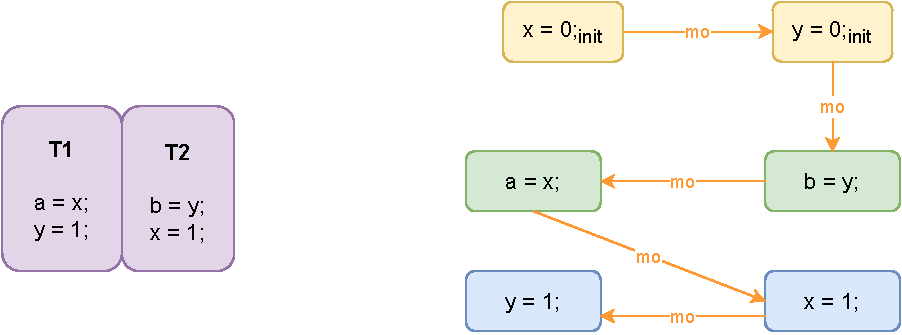
\includegraphics[scale=0.7]{4.ECMAScriptMemoryModel/MemoryOrder.pdf}
            \caption{An example with a memory order (total) among all events.}
        \end{figure}

    \critic{blue}{An interesting part is that memory order, though total, is a bit undefined as to how it weaves together this total order given different init events. One can certainly make init events weaved among events that occur in each agent, thus making it sort of subjective as to when certain memory fragments are initialized. Discuss with Clark.}